\chapter{Schematics}
\labch{schematics}
\section{Power Amplifier}
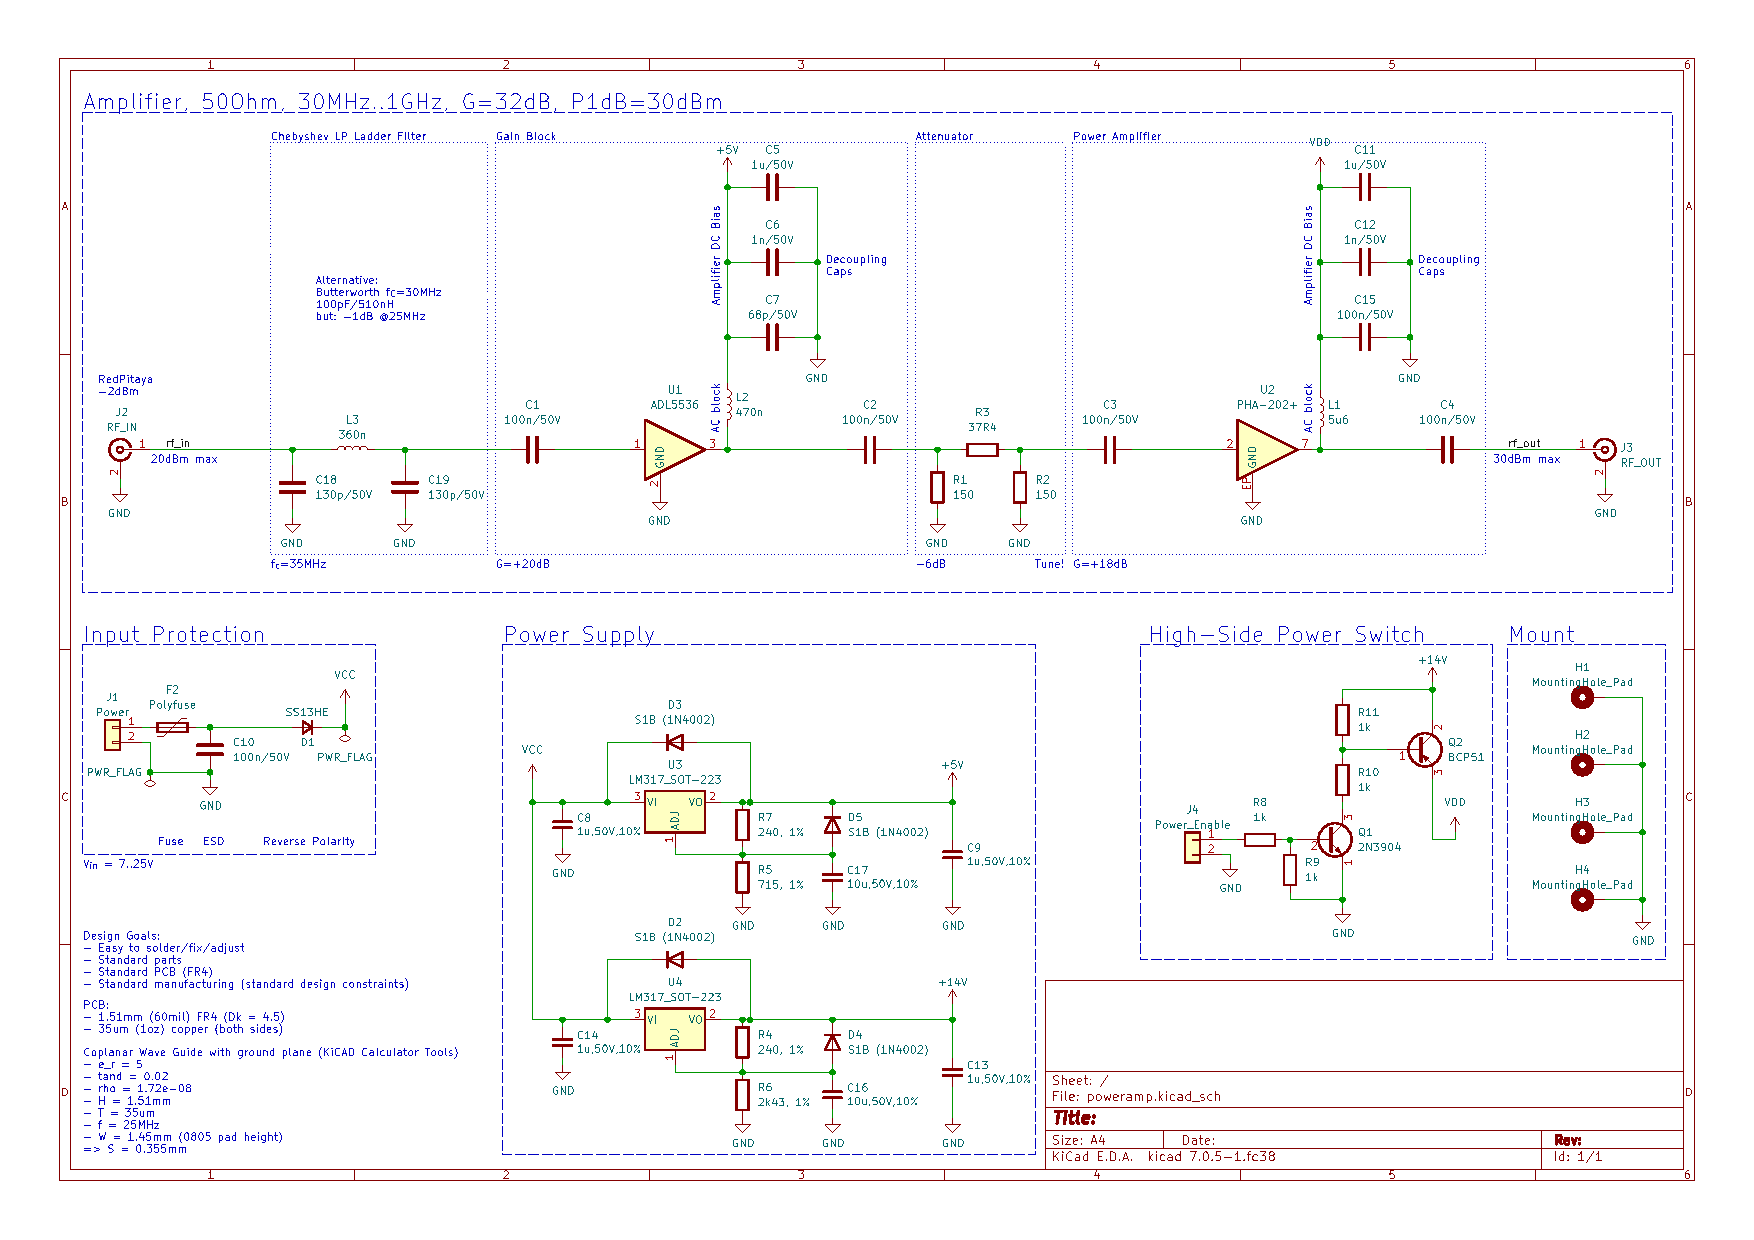
\includegraphics[angle=90,width=0.9\textwidth]{poweramp.pdf}

\section{Switch}
\labsec{switch-schematic}
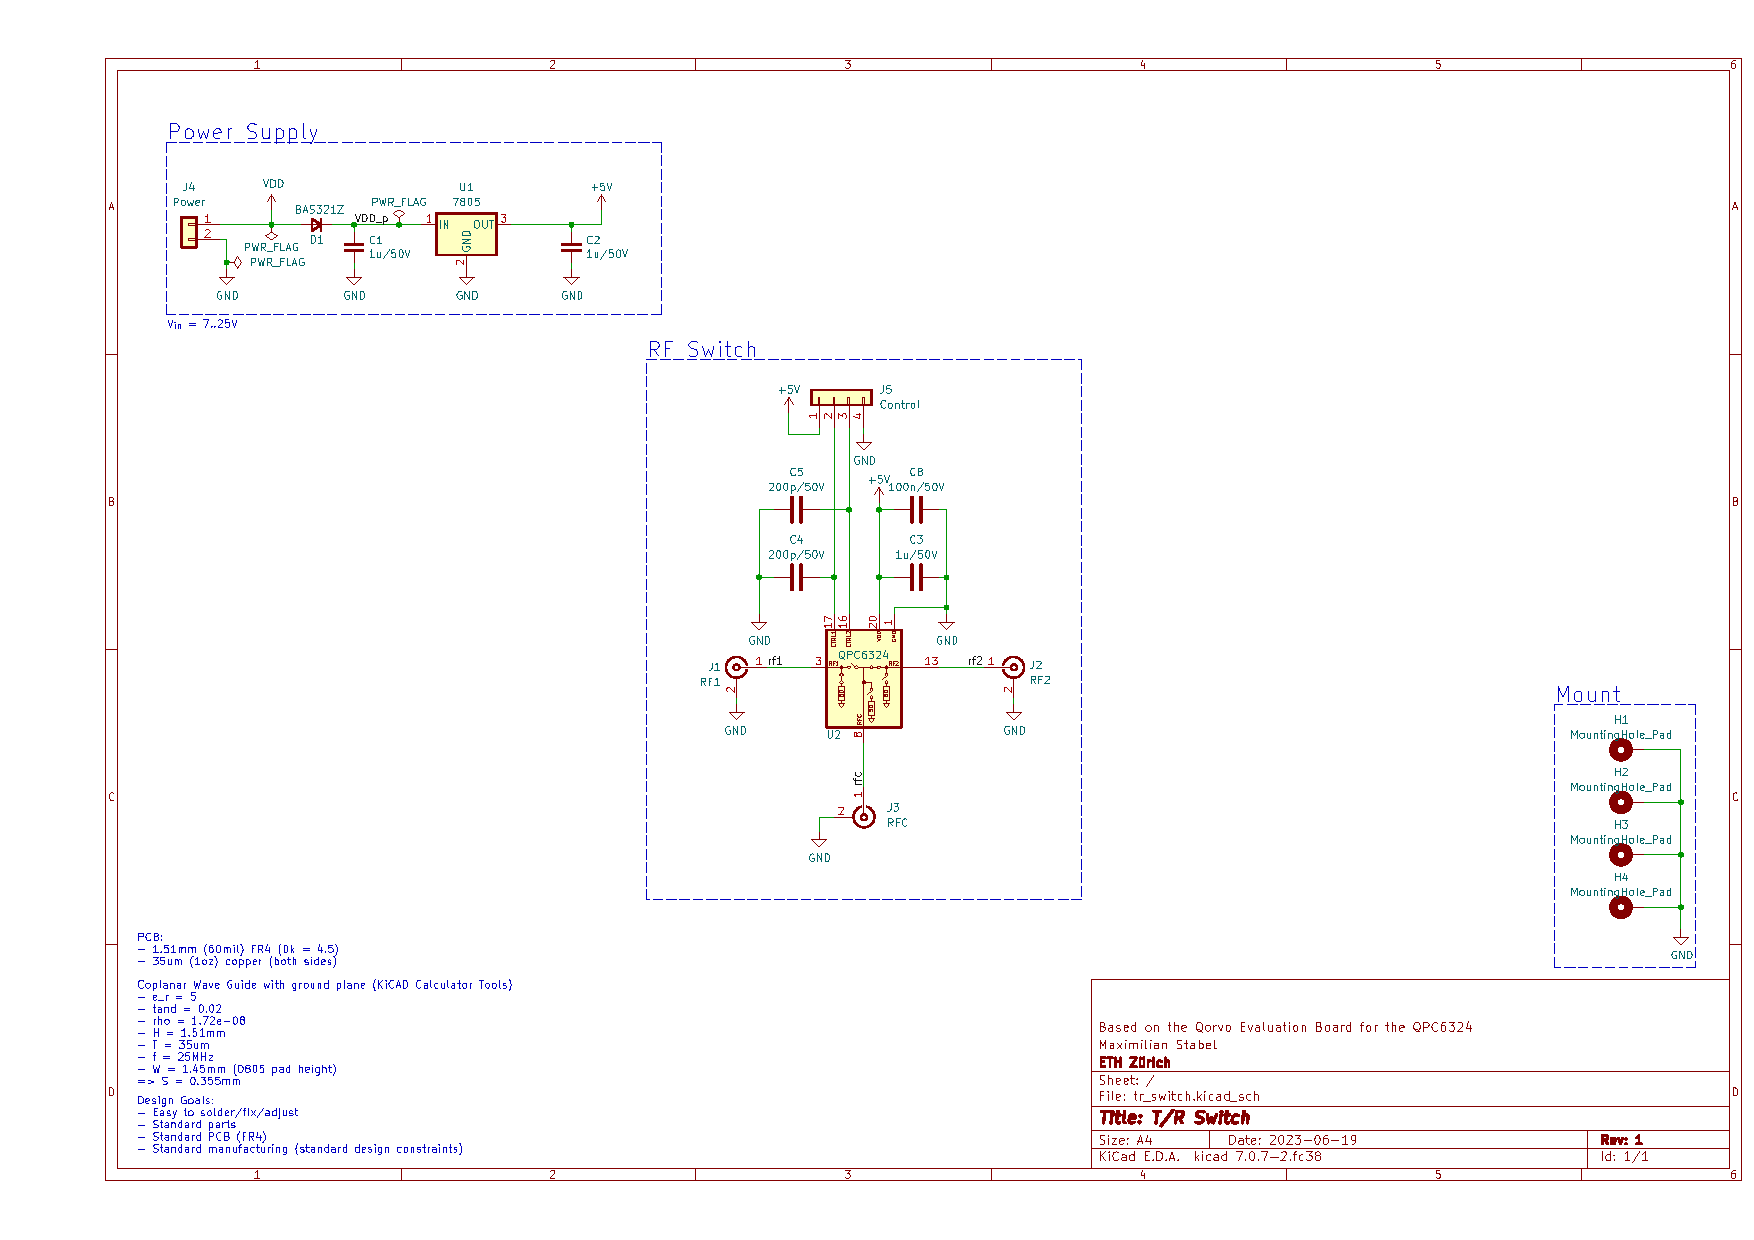
\includegraphics[angle=90,width=\textwidth]{tr_switch.pdf}

\section{Low Noise Amplifier}
\labsec{lna-schematic}
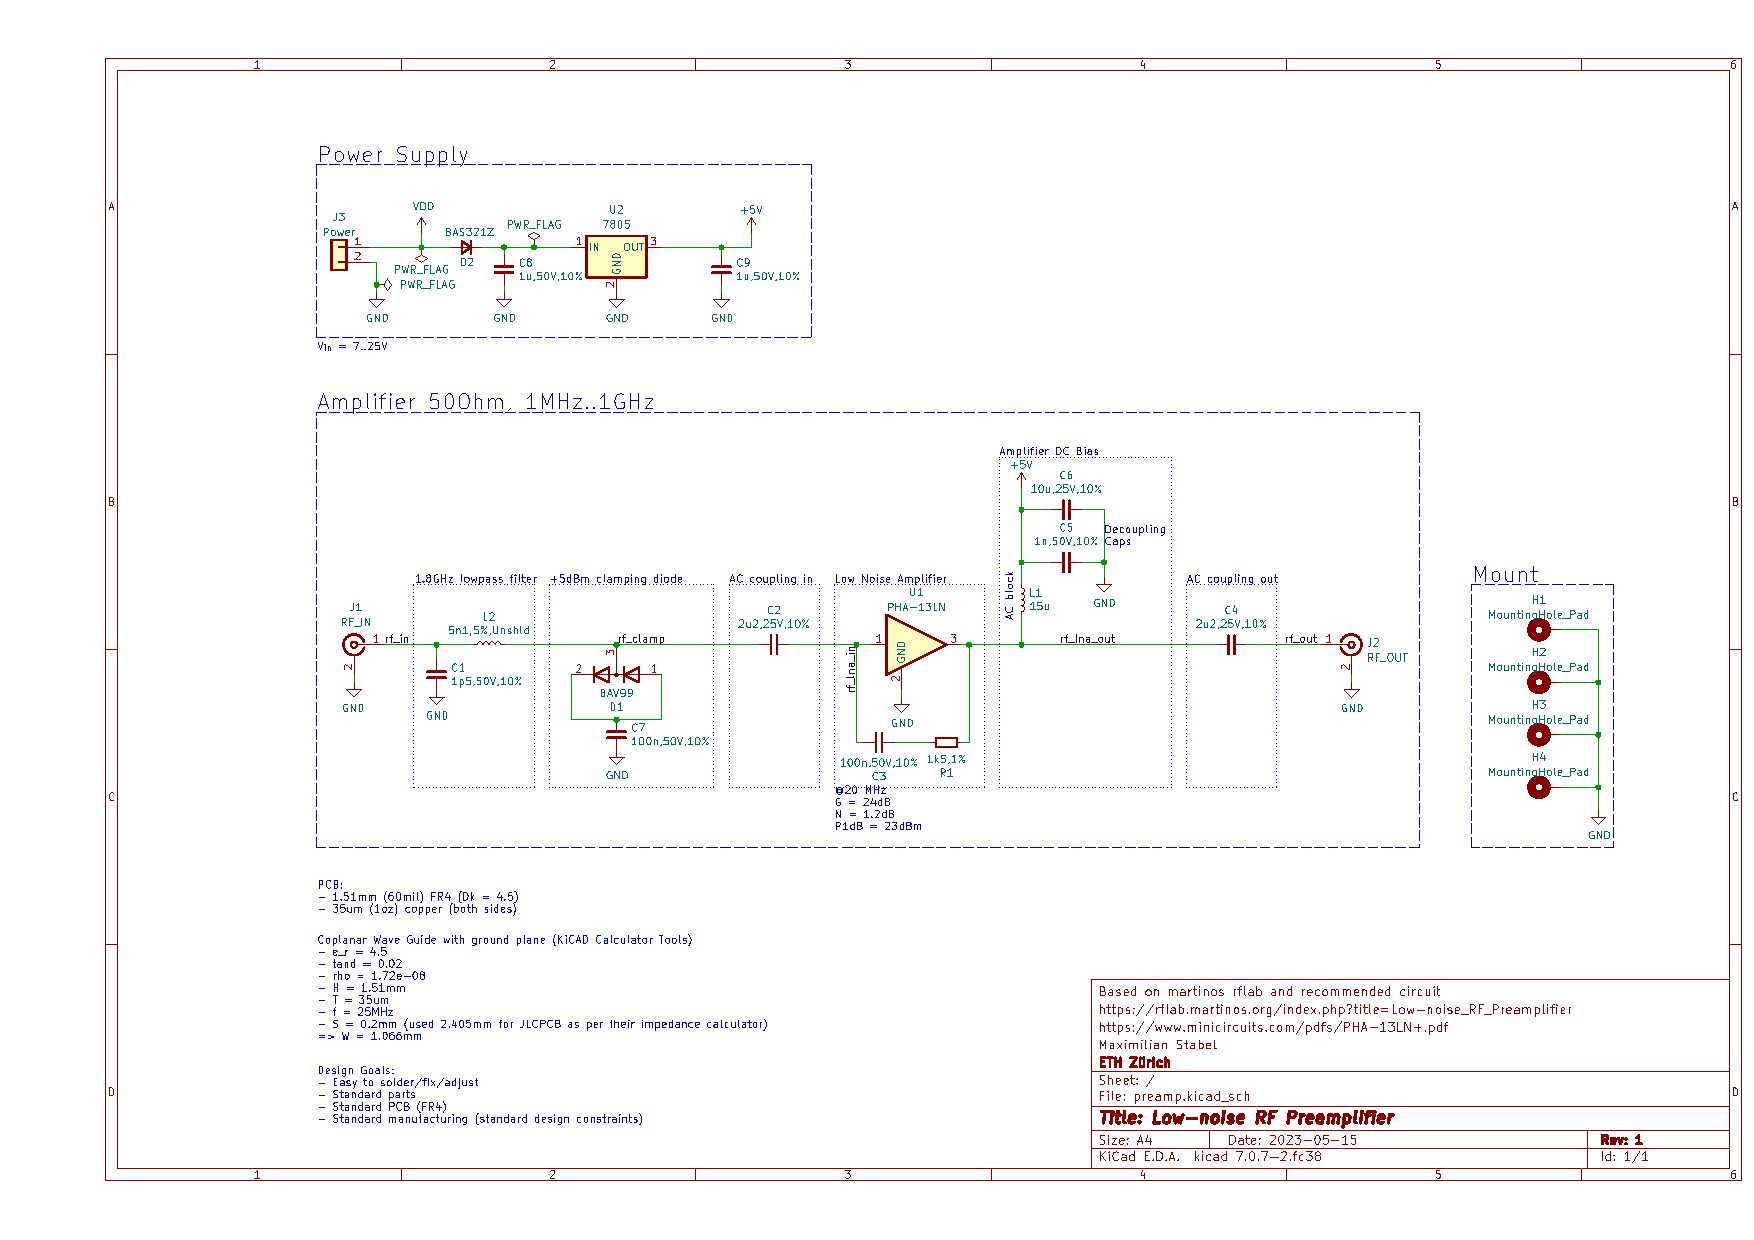
\includegraphics[angle=90,width=\textwidth]{preamp.pdf}

\section{32-channel current source}
\labsec{32-channel-current-source-schematic}
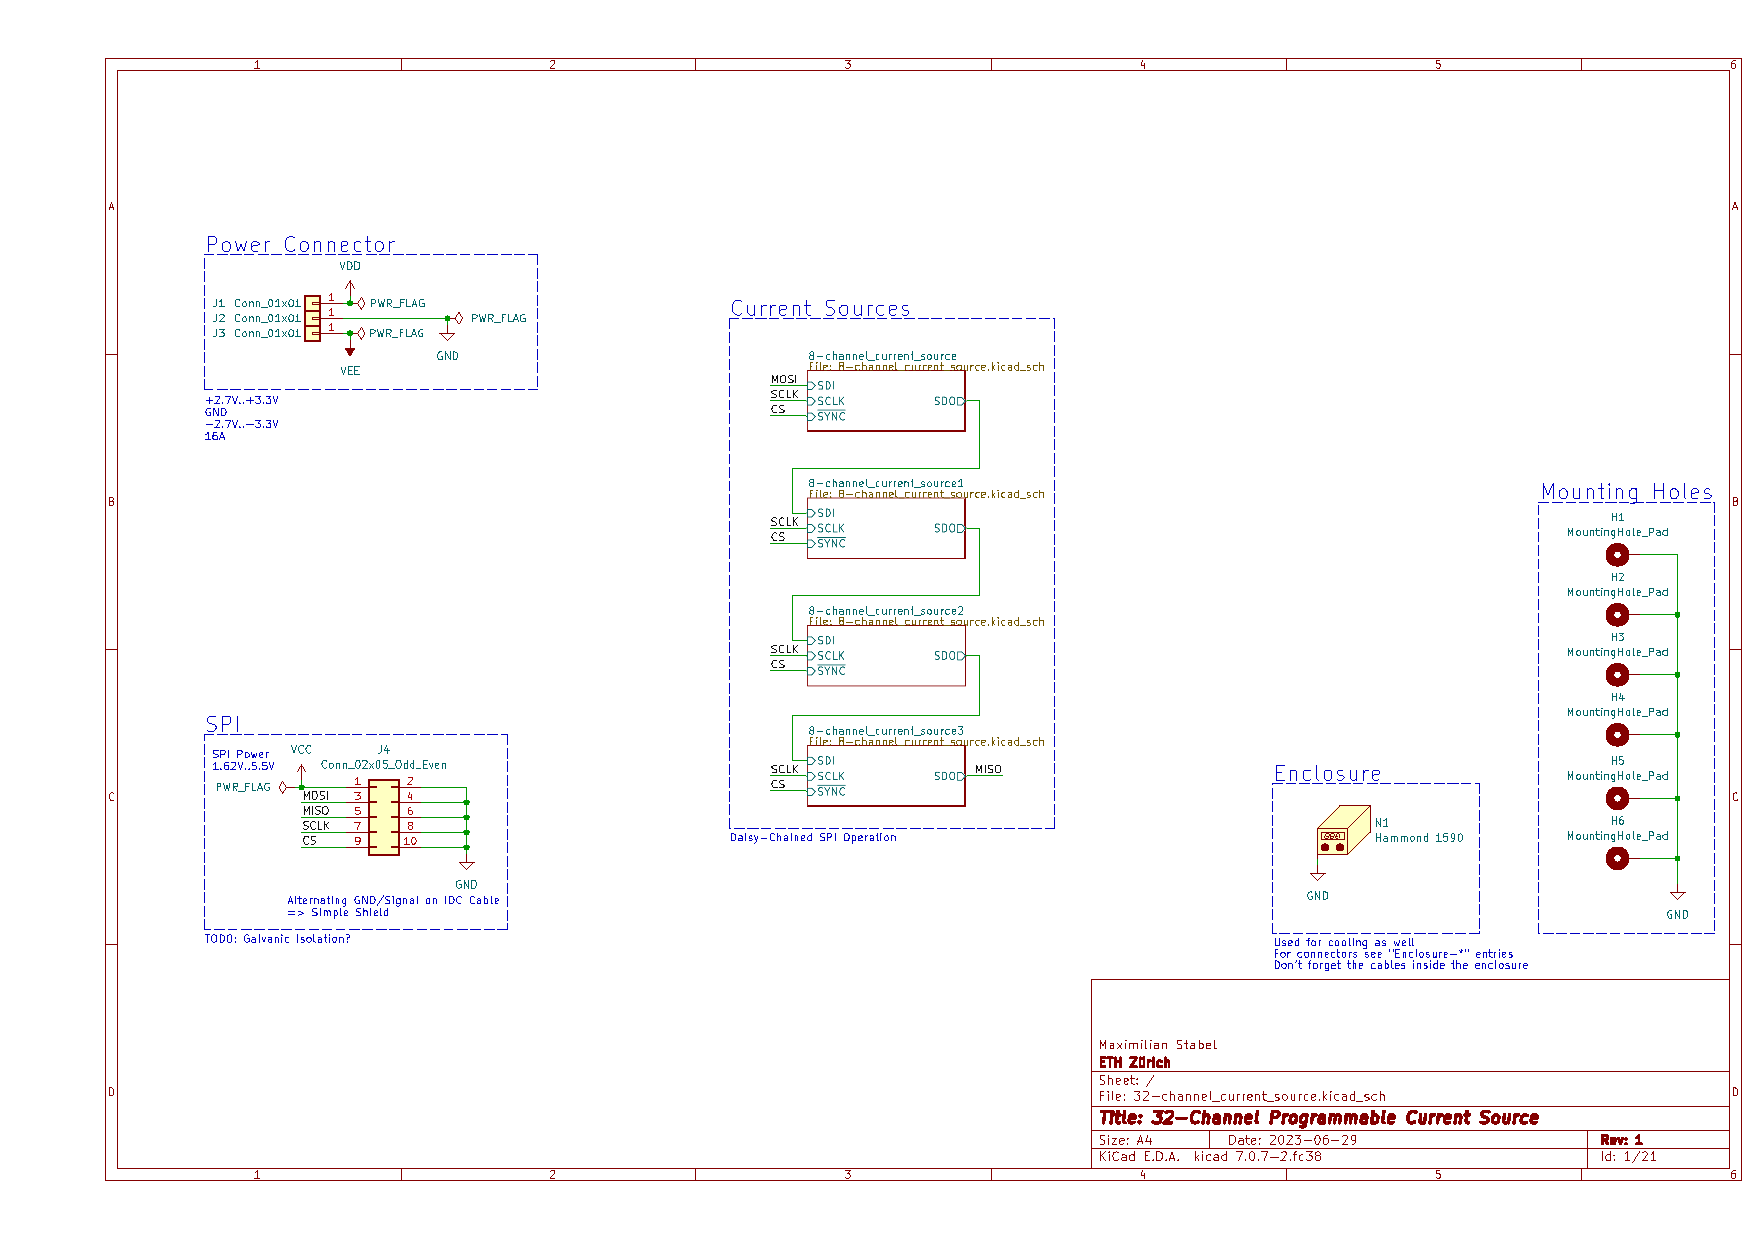
\includegraphics[angle=90,width=\textwidth,page=1]{32-channel_current_source.pdf}

\includegraphics[angle=90,width=\textwidth,page=2]{32-channel_current_source.pdf}

\includegraphics[angle=90,width=\textwidth,page=3]{32-channel_current_source.pdf}

% \chapter{About this thesis}
% \labch{about}

% This thesis was heavily influenced by Jean-Luc Doumont's \enquote{English Communication for Scientists} \sidecite{doumontEnglishCommunicationScientists2010}.

% \chapter{Schematics}

